% questions.tex —— 2013 年全国Ⅱ卷（文科） · 题目内容片段（无答案）
% 由 tools/generate_projects.py 依来源总账自 2013/2013_数学真题_全国2文_试题.md 生成，勿手改（改源 MD 后重跑）


\gkpart{数学}

\begin{gktip}
\textbf{来源说明}：本题面依据固定源 PDF 两页 A3 题面逐题转录，原卷印刷页码 831–832。固定源只含试题和作答空白，不附答案或解析；答案和解析均由本库独立复算。

\textbf{图形说明}：第 7、9、18、19、22 题的题面图形在 LaTeX 工程中以 TikZ 矢量源重绘。题面中的图片标记仅为转换器定位这些矢量源的标记，仓库不保存 PNG、JPEG 或 SVG 图形文件。
\end{gktip}

\gkpart{一、选择题}

\begin{question}
\gkti{1}已知集合 $M=\{x\mid-3<x<1\}$，$N=\{-3,-2,-1,0,1\}$，则 $M\cap N=$\mbox{（　　）}

（A）$\{-2,-1,0,1\}$　　（B）$\{-3,-2,-1,0\}$　　（C）$\{-2,-1,0\}$　　（D）$\{-3,-2,-1\}$

\end{question}
\begin{question}
\gkti{2}$\left|\dfrac{2}{1+i}\right|=$\mbox{（　　）}

（A）$2\sqrt2$　　（B）$2$　　（C）$\sqrt2$　　（D）$1$

\end{question}
\begin{question}
\gkti{3}设 $x,y$ 满足约束条件

\nopagebreak[4]
\[
\begin{cases}
x-y+1\geqslant0,\\
x+y-1\geqslant0,\\
x\leqslant3,
\end{cases}
\]

则 $z=2x-3y$ 的最小值是\mbox{（　　）}

（A）$-7$　　（B）$-6$　　（C）$-5$　　（D）$-3$

\end{question}
\begin{question}
\gkti{4}$\triangle ABC$ 的内角 $A,B,C$ 的对边分别为 $a,b,c$，已知 $b=2$，$B=\dfrac\pi6$，$C=\dfrac\pi4$，则 $\triangle ABC$ 的面积为\mbox{（　　）}

（A）$2\sqrt3+2$　　（B）$\sqrt3+1$　　（C）$2\sqrt3-2$　　（D）$\sqrt3-1$

\end{question}
\begin{question}
\gkti{5}设椭圆 $C:\dfrac{x^2}{a^2}+\dfrac{y^2}{b^2}=1\ (a>b>0)$ 的左、右焦点分别为 $F_1,F_2$，$P$ 是 $C$ 上的点，$PF_2\perp F_1F_2$，$\angle PF_1F_2=30^\circ$，则 $C$ 的离心率为\mbox{（　　）}

（A）$\dfrac{\sqrt3}{6}$　　（B）$\dfrac13$　　（C）$\dfrac12$　　（D）$\dfrac{\sqrt3}{3}$

\end{question}
\begin{question}
\gkti{6}已知 $\sin2\alpha=\dfrac23$，则 $\cos^2\left(\alpha+\dfrac\pi4\right)=$\mbox{（　　）}

（A）$\dfrac16$　　（B）$\dfrac13$　　（C）$\dfrac12$　　（D）$\dfrac23$

\Needspace{0.4\textheight}
\end{question}
\begin{question}
\gkti{7}执行如图的程序框图，如果输入的 $N=4$，那么输出的 $S=$\mbox{（　　）}
\nopagebreak[4]
\begin{center}% 2013 全国卷Ⅱ文科第 7 题：阶乘倒数累加程序框图。
\begin{tikzpicture}[font=\footnotesize, >=Stealth, node distance=4mm, line width=0.4pt,
  box/.style={draw, minimum height=1.65em, minimum width=8.0em, inner xsep=4pt},
  term/.style={draw, rounded corners=6pt, minimum height=1.65em, inner xsep=8pt},
  io/.style={draw, trapezium, trapezium left angle=70, trapezium right angle=110,
             minimum height=1.65em, inner xsep=4pt},
  dec/.style={draw, diamond, aspect=2.25, inner sep=1.6pt}]
  \node[term] (start) {开始};
  \node[io, below=of start] (input) {输入 $N$};
  \node[box, below=of input] (init) {$k=1,\ S=0,\ T=1$};
  \node[box, below=of init] (divide) {$T=\dfrac{T}{k}$};
  \node[box, below=of divide] (sum) {$S=S+T$};
  \node[box, below=of sum] (inc) {$k=k+1$};
  \node[dec, below=7mm of inc] (cond) {$k>N$};
  \node[io, below=8mm of cond] (output) {输出 $S$};
  \node[term, below=of output] (end) {结束};
  \draw[->] (start)--(input)--(init)--(divide)--(sum)--(inc)--(cond);
  \draw[->] (cond.south)--node[right] {是}(output);
  \draw[->] (output)--(end);
  \draw[->] (cond.east)-| node[pos=0.18,above] {否} ($(divide.east)+(12mm,0)$) |- (divide.east);
\end{tikzpicture}
\end{center}
\nopagebreak[4]
（A）$1+\dfrac12+\dfrac13+\dfrac14$　　（B）$1+\dfrac12+\dfrac1{3\times2}+\dfrac1{4\times3\times2}$

（C）$1+\dfrac12+\dfrac13+\dfrac14+\dfrac15$　　（D）$1+\dfrac12+\dfrac1{3\times2}+\dfrac1{4\times3\times2}+\dfrac1{5\times4\times3\times2}$

\end{question}
\begin{question}
\gkti{8}设 $a=\log_3 2$，$b=\log_5 2$，$c=\log_2 3$，则\mbox{（　　）}

（A）$a>c>b$　　（B）$b>c>a$　　（C）$c>b>a$　　（D）$c>a>b$

\Needspace{0.4\textheight}
\end{question}
\begin{question}
\gkti{9}一个四面体的顶点在空间直角坐标系 $O-xyz$ 中的坐标分别是 $(1,0,1)$，$(1,1,0)$，$(0,1,1)$，$(0,0,0)$，画该四面体三视图中的正视图时，以 $zOx$ 平面为投影面，则得到正视图可以为\mbox{（　　）}
\nopagebreak[4]
\begin{center}% 2013 全国卷Ⅱ文科第 9 题：四面体正视图的四个选项；虚线表示隐藏棱。
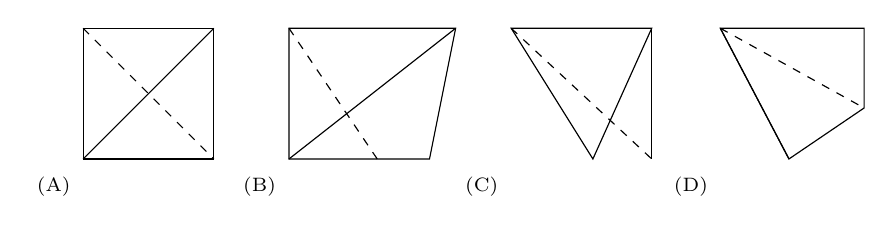
\begin{tikzpicture}[font=\scriptsize, line width=0.42pt, scale=0.83]
  % A
  \begin{scope}
    \node at (-0.45,-0.42) {(A)};
    \draw (0,0)--(2,0)--(2,2)--(0,2)--cycle;
    \draw (0,0)--(2,2);
    \draw[dashed] (0,2)--(2,0);
  \end{scope}
  % B
  \begin{scope}[xshift=3.15cm]
    \node at (-0.45,-0.42) {(B)};
    \draw (0,0)--(2.15,0)--(2.55,2)--(0,2)--cycle;
    \draw (0,0)--(2.55,2);
    \draw[dashed] (0,2)--(1.35,0);
  \end{scope}
  % C
  \begin{scope}[xshift=6.55cm]
    \node at (-0.45,-0.42) {(C)};
    \draw (0,2)--(2.15,2)--(1.25,0)--cycle;
    \draw (2.15,2)--(2.15,0);
    \draw[dashed] (0,2)--(2.15,0);
  \end{scope}
  % D
  \begin{scope}[xshift=9.75cm]
    \node at (-0.45,-0.42) {(D)};
    \draw (0,2)--(2.20,2)--(2.20,0.78)--(1.05,0)--cycle;
    \draw (0,2)--(1.05,0);
    \draw[dashed] (0,2)--(2.20,0.78);
  \end{scope}
\end{tikzpicture}
\end{center}
\nopagebreak[4]
\end{question}
\begin{question}
\gkti{10}设抛物线 $C:y^2=4x$ 的焦点为 $F$，直线 $l$ 过 $F$ 且与 $C$ 交于 $A,B$ 两点，若 $|AF|=3|BF|$，则 $l$ 的方程为\mbox{（　　）}

（A）$y=x-1$ 或 $y=-x+1$　　（B）$y=\dfrac{\sqrt3}{3}(x-1)$ 或 $y=-\dfrac{\sqrt3}{3}(x-1)$

（C）$y=\sqrt3(x-1)$ 或 $y=-\sqrt3(x-1)$　　（D）$y=\dfrac{\sqrt2}{2}(x-1)$ 或 $y=-\dfrac{\sqrt2}{2}(x-1)$

\end{question}
\begin{question}
\gkti{11}已知函数 $f(x)=x^3+ax^2+bx+c$，下列结论中错误的是\mbox{（　　）}

（A）$\exists x_0\in\mathbb R,\ f(x_0)=0$

（B）函数 $y=f(x)$ 的图象是中心对称图形

（C）若 $x_0$ 是 $f(x)$ 的极小值点，则 $f(x)$ 在区间 $(-\infty,x_0)$ 单调递减

（D）若 $x_0$ 是 $f(x)$ 的极值点，则 $f'(x_0)=0$

\end{question}
\begin{question}
\gkti{12}若存在正数 $x$ 使 $2^x(x-a)<1$ 成立，则 $a$ 的取值范围是\mbox{（　　）}

（A）$(-\infty,+\infty)$　　（B）$(-2,+\infty)$　　（C）$(0,+\infty)$　　（D）$(-1,+\infty)$

\end{question}
\gkpart{二、填空题}

\begin{question}
\gkti{13}从 $1,2,3,4,5$ 中任意取出两个不同的数，其和为 $5$ 的概率是\gkblank{}。

\end{question}
\begin{question}
\gkti{14}已知正方形 $ABCD$ 的边长为 $2$，$E$ 为 $CD$ 的中点，则 $\overrightarrow{AE}\cdot\overrightarrow{BD}=$\gkblank{}。

\end{question}
\begin{question}
\gkti{15}已知正四棱锥 $O-ABCD$ 的体积为 $\dfrac{3\sqrt2}{2}$，底面边长为 $\sqrt3$，则以 $O$ 为球心，$OA$ 为半径的球的表面积为\gkblank{}。

\end{question}
\begin{question}
\gkti{16}函数 $y=\cos(2x+\varphi)\ (-\pi\leqslant\varphi<\pi)$ 的图象向右平移 $\dfrac\pi2$ 个单位后，与函数 $y=\sin\left(2x+\dfrac\pi3\right)$ 的图象重合，则 $\varphi=$\gkblank{}。

\end{question}
\gkpart{三、解答题}

\begin{question}
\gkti{17}已知等差数列 $\{a_n\}$ 的公差不为零，$a_1=25$，且 $a_1,a_{11},a_{13}$ 成等比数列。

(1) 求 $\{a_n\}$ 的通项公式；

(2) 求 $a_1+a_4+a_7+\cdots+a_{3n-2}$。

\Needspace{0.4\textheight}
\end{question}
\begin{question}
\gkti{18}如图，直三棱柱 $ABC-A_1B_1C_1$ 中，$D,E$ 分别是 $AB,BB_1$ 的中点。
\nopagebreak[4]
\begin{center}% 2013 全国卷Ⅱ文科第 18 题：直三棱柱 ABC-A_1B_1C_1，D、E 为给定中点。
\begin{tikzpicture}[font=\footnotesize, line width=0.45pt]
  \coordinate (A) at (0,0);
  \coordinate (B) at (1.05,-1.05);
  \coordinate (C) at (4.10,0);
  \coordinate (A1) at (0,3.60);
  \coordinate (B1) at (2.05,1.85);
  \coordinate (C1) at (4.10,3.60);
  \coordinate (D) at ($(A)!0.5!(B)$);
  \coordinate (E) at ($(B)!0.5!(B1)$);
  \draw (A)--(A1)--(C1)--(C)--cycle;
  \draw (A1)--(B1)--(C1);
  \draw (B)--(B1);
  \draw (A1)--(D)--(C);
  \draw (A1)--(E)--(C);
  \draw[dashed] (A)--(B)--(C) (D)--(E) (A1)--(C);
  \node[below left] at (A) {$A$};
  \node[below] at (B) {$B$};
  \node[below right] at (C) {$C$};
  \node[above left] at (A1) {$A_1$};
  \node[above] at (B1) {$B_1$};
  \node[above right] at (C1) {$C_1$};
  \node[below left] at (D) {$D$};
  \node[left] at (E) {$E$};
\end{tikzpicture}
\end{center}
\nopagebreak[4]
(1) 证明：$BC_1\parallel$ 平面 $A_1CD$；

(2) 设 $AA_1=AC=CB=2$，$AB=2\sqrt2$，求三棱锥 $C-A_1DE$ 的体积。

<!-- 固定源 PDF 第 1 页（印刷页 831）至此。 -->

\Needspace{0.4\textheight}
\end{question}
\begin{question}
\gkti{19}经销商经销某种农产品，在一个销售季度内，每售出 $1\ \mathrm t$ 该产品获利润 $500$ 元，未售出的产品，每 $1\ \mathrm t$ 亏损 $300$ 元。根据历史资料，得到销售季度内市场需求量的频率分布直方图，如图所示。经销商为下一个销售季度购进了 $130\ \mathrm t$ 该农产品。以 $X$（单位：$\mathrm t$，$100\leqslant X\leqslant150$）表示下一个销售季度内的市场需求量，$T$（单位：元）表示下一个销售季度内经销该农产品的利润。
\nopagebreak[4]
\begin{center}% 2013 全国卷Ⅱ文科第 19 题：频率分布直方图。
\begin{tikzpicture}[font=\footnotesize, >=Stealth, line width=0.42pt, x=0.18cm, y=105cm]
  \draw[->] (-12,0)--(58,0) node[right,align=center] {市场需求量};
  \draw[->] (-10,0)--(-10,0.038) node[above,align=center] {频率\\组距};
  % 坐标轴在 0 与 100 之间的截断符号。
  \draw (-7.8,0.0007)--(-7.0,-0.0007)--(-6.2,0.0007)--(-5.4,-0.0007)--(-4.6,0.0007);
  \draw[dashed] (-10,0.010)--(0,0.010); \node[left,xshift=-1mm] at (-10,0.010) {0.010};
  \draw[dashed] (-10,0.015)--(40,0.015); \node[left,xshift=-1mm] at (-10,0.015) {0.015};
  \draw[dashed] (-10,0.020)--(10,0.020); \node[left,xshift=-1mm] at (-10,0.020) {0.020};
  \draw[dashed] (-10,0.025)--(30,0.025); \node[left,xshift=-1mm] at (-10,0.025) {0.025};
  \draw[dashed] (-10,0.030)--(20,0.030); \node[left,xshift=-1mm] at (-10,0.030) {0.030};
  \draw (0,0) rectangle (10,0.010);
  \draw (10,0) rectangle (20,0.020);
  \draw (20,0) rectangle (30,0.030);
  \draw (30,0) rectangle (40,0.025);
  \draw (40,0) rectangle (50,0.015);
  \node[below] at (-10,0) {$0$};
  \foreach \x/\lab in {0/100,10/110,20/120,30/130,40/140,50/150}
    \node[below] at (\x,0) {\lab};
\end{tikzpicture}
\end{center}
\nopagebreak[4]
(1) 将 $T$ 表示为 $X$ 的函数；

(2) 根据直方图估计利润 $T$ 不少于 $57000$ 元的概率。

\end{question}
\begin{question}
\gkti{20}在平面直角坐标系 $xOy$ 中，已知圆 $P$ 在 $x$ 轴上截得线段长为 $2\sqrt2$，在 $y$ 轴上截得线段长为 $2\sqrt3$。

(1) 求圆心 $P$ 的轨迹方程；

(2) 若 $P$ 点到直线 $y=x$ 的距离为 $\dfrac{\sqrt2}{2}$，求圆 $P$ 的方程。

\end{question}
\begin{question}
\gkti{21}已知函数 $f(x)=x^2e^{-x}$。

(1) 求 $f(x)$ 的极小值和极大值；

(2) 当曲线 $y=f(x)$ 的切线 $l$ 的斜率为负数时，求 $l$ 在 $x$ 轴上截距的取值范围。

\Needspace{0.4\textheight}
\end{question}
\begin{question}
\gkti{22}如图，$CD$ 为 $\triangle ABC$ 外接圆的切线，$AB$ 的延长线交直线 $CD$ 于点 $D$，$E,F$ 分别为弦 $AB$ 与弦 $AC$ 上的点，且 $BC\cdot AE=DC\cdot AF$，$B,E,F,C$ 四点共圆。
\nopagebreak[4]
\begin{center}% 2013 全国卷Ⅱ文科第 22 题：外接圆、切线及过 B,E,F,C 的圆。
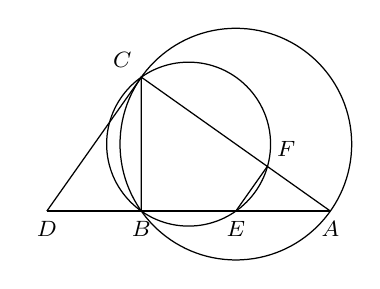
\begin{tikzpicture}[font=\footnotesize, line width=0.45pt]
  \coordinate (B) at (0,0);
  \coordinate (E) at (1.20,0);
  \coordinate (A) at (2.40,0);
  \coordinate (D) at (-1.20,0);
  \coordinate (C) at (0,1.70);
  \coordinate (F) at (1.60,0.567);
  \coordinate (O) at (1.20,0.85);
  \coordinate (o) at (0.60,0.85);
  \draw (O) circle[radius=1.471];
  \draw (o) circle[radius=1.041];
  \draw (D)--(A);
  \draw (D)--(C);
  \draw (B)--(C)--(A);
  \draw (E)--(F);
  \node[below] at (D) {$D$};
  \node[below] at (B) {$B$};
  \node[below] at (E) {$E$};
  \node[below] at (A) {$A$};
  \node[above left] at (C) {$C$};
  \node[above right] at (F) {$F$};
\end{tikzpicture}
\end{center}
\nopagebreak[4]
(1) 证明：$CA$ 是 $\triangle ABC$ 外接圆的直径；

(2) 若 $DB=BE=EA$，求过 $B,E,F,C$ 四点的圆的面积与 $\triangle ABC$ 外接圆面积的比值。

\end{question}
\begin{question}
\gkti{23}已知动点 $P,Q$ 都在曲线 $C:\begin{cases}x=2\cos t,\\y=2\sin t,\end{cases}\ (t$ 为参数$)$ 上，对应参数分别为 $t=\alpha$ 与 $t=2\alpha\ (0<\alpha<2\pi)$，$M$ 为 $PQ$ 的中点。

(1) 求 $M$ 的轨迹的参数方程；

(2) 将 $M$ 到坐标原点的距离 $d$ 表示为 $\alpha$ 的函数，并判断 $M$ 的轨迹是否经过坐标原点。

\end{question}
\begin{question}
\gkti{24}设 $a,b,c$ 均为正数，且 $a+b+c=1$，证明：

(1) $ab+bc+ca\leqslant\dfrac13$；

(2) $\dfrac{a^2}{b}+\dfrac{b^2}{c}+\dfrac{c^2}{a}\geqslant1$。

\end{question}